\def\micro{\mu m}
\def\um{$\micro$ }
\def\degreesC{$\degree C$ }
\def\percent{$\%$ }
\documentclass[10pt,a4paper,oneside]{article}
\usepackage[left=2cm,right=2cm,top=2cm,bottom=2cm]{geometry}

\input{../global_color_scheme.tex}
\usepackage[utf8]{inputenc}
\usepackage[english]{babel}
\usepackage{forloop}
\usepackage{amsmath}
\usepackage{amsfonts}
\usepackage{amssymb}
\usepackage{gensymb}
\usepackage{mdframed}
\usepackage{graphicx}
\usepackage{tikz}
\usetikzlibrary{arrows,automata,shapes}
\usepackage[siunitx]{circuitikz}
\usepackage{makecell}
\usepackage{array}

\def\WaferClean{
\begin{tikzpicture}\node [fill=cyan, rounded corners=5pt] {Clean};\end{tikzpicture}}
\def\WaferSemiClean{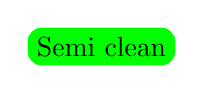
\begin{tikzpicture}\node [fill=green, rounded corners=5pt] {Semi clean};\end{tikzpicture}}
\def\WaferNonStandard{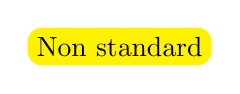
\begin{tikzpicture}\node [fill=yellow, rounded corners=5pt] {Non standard};\end{tikzpicture}}

\usepackage[colorlinks=true,linkcolor=blue,urlcolor=black,bookmarksopen=true]{hyperref}
\usepackage{bookmark}
\usepackage{hyperref}
\usepackage{sepfootnotes}
\usepackage{lipsum,tocloft} 
\usetikzlibrary{positioning}
\usetikzlibrary{patterns}

\usepackage{float}
\floatstyle{boxed} 
\restylefloat{figure}

\title{Libre Silicon process design rules}
\date{\today}
\author{
  David Lanzendörfer
  \and
  Hagen Sankowski
}

\makeindex

\newcounter{ct}
\def\CrossSectionOnly{0.3}
\def\CrossAndTopSection{0.2}
\def\CrossAndTopSectionBig{0.3}
\def\VLSILayout{0.4}

\DeclareMathOperator\erfc{erfc}

\setlength{\parindent}{0pt} % get rid of annoying indents

\begin{document}
\begin{abstract}
	Copyright © 2017 LANCEVILLE TECHNOLOGY GROUP CO., LIMITED. All rights reserved. \\

This process is licensed under the Libre Silicon public license; you can redistribute it and/or modify it under the terms of the Libre Silicon public license
as published by the Libre Silicon alliance, either version 1 of the License, or (at your option) any later version.

This design is distributed in the hope that it will be useful, but WITHOUT ANY WARRANTY; without even the implied warranty of MERCHANTABILITY or FITNESS FOR A PARTICULAR PURPOSE.
See the Libre Silicon Public License for more details. \\

This document is part of the specification of the free silicon manufacturing standard for manufacturing the LibreSilicon standard logic cells\footnote{\url{https://git.libresilicon.com/?p=redmine/standard-cell-lib.git;a=summary}} and related free technology nodes from the LibreSilicon project.

For this initial revision 0.1 a gate-first approach has been chosen which led to the choice of polysilicon as the gate electrode material because of the simplicity of the gate alignment.
For better isolation properties of the transistors and gates in overall a box-isolation approach has been chosen.
All of these choices have been made with the future scale down from the recent $1 \mu m$ to smaller structure sizes.
\textbf{This process is for manufacturing $1 \mu m$ only!}
But further releases which will have been tested with smaller structure sizes can be expected.

\end{abstract}
\newpage
\maketitle
\section{Layer Definitions}\label{design_rules_layer_definitions}

\begin{center}
%    \captionof{table}{Mask Layers (for Production)}
    \begin{tabular}{|l|c|c|p{7.5cm}|}
    \hline
        \textbf{Name} & \textbf{GDSII} & \textbf{CIF} & \textbf{Description} \\
    \hline
        PWELL   & 41 & CWP & p-well \\
        NWELL   & 42 & CWN & n-well \\
        ACTIVE  & 43 & CAA & active area \\
        PPLUS   & 44 & CSP & $p^{+}$ implant \\
        NPLUS   & 45 & CSN & $n^{+}$ implant \\
        POLY    & 46 & CPG & poly silicium \\
        CONTACT & 25 & CCC & contact (connects METAL1 to POLY) \\
        METAL1  & 49 & CM1 & lowest metal layer \\
        VIA1    & 50 & CV1 & via layer (connects METAL2 to METAL1) \\
        METAL2  & 51 & CM2 & second metal layer \\
        VIA2    & 61 & CV2 & via layer (connects METAL3 to METAL2) \\
        METAL3  & 62 & CM3 & third metal layer \\
        GLASS   & 52 & COG & passivation / isolation \\
    \hline
    \end{tabular}
\end{center}

\section{General Requirements}\label{design_rules_general_requirements}

\begin{flushleft}
    \begin{tabular}{c p{9cm} c}
        1.1  & All scaled dimensions are specified in Lambda & $\lambda$. \\
        1.2  & All fixed dimensions are specified in Microns & $\mu m$. \\
        1.3  & All geometries must be drawn on grid. The grid size is & $1 \lambda$. \\
        1.4  & Polygones should be rectangles with 90 degree angles only. \\
        1.5  & The die size should be an integer multiple of & $10 \mu m$. \\
    \end{tabular}
\end{flushleft}


\begin{center}
    \begin{tabular}{|l|c|c|}
    \hline
        \textbf{Node} & \textbf{$\lambda$} & \textbf{$2 \lambda$} \\
    \hline
	    1 micron & 500nm & 1$\mu$m \\
	    0.5 micron & 250nm & 500nm \\
	    0.25 micron & 125nm & 250nm \\
    \hline
    \end{tabular}
\end{center}

\section{Process Layer Overview}\label{design_rules_process_layer_overview}

\begin{center}
%    \captionof{table}{Mask Layer Minimum Values}
    \begin{tabular}{|l|c|c|}
    \hline
        \textbf{Name} & \textbf{Minimum Width} & \textbf{Minimum Spacing} \\
    \hline
        PWELL   & 10 $\lambda$ & 10 $\lambda$ \\
        NWELL   & 10 $\lambda$ & 10 $\lambda$ \\
        ACTIVE  & 3  $\lambda$ & 3  $\lambda$ \\
        POLY    & 2  $\lambda$ & 2  $\lambda$ \\
        CONTACT & 2  $\lambda$ & 2  $\lambda$ \\
        METAL1  & 4  $\lambda$ & 4  $\lambda$ \\
        VIA1    & 2  $\lambda$ & 3  $\lambda$ \\
        METAL2  & 4  $\lambda$ & 4  $\lambda$ \\
        VIA2    & 2  $\lambda$ & 3  $\lambda$ \\
        METAL3  & 6  $\lambda$ & 4  $\lambda$ \\
    \hline
    \end{tabular}
\end{center}

\section{Structure Rules}\label{design_rules_structure_rules}

\subsection{PWELL Rules}\label{design_rules_pwell_rules}

\begin{center}
    \begin{tikzpicture}[scale=(.33)]
        \filldraw[fill=pwell] (0, 0) rectangle ++(10, 10) node[near end] {PWELL};
        \draw[<->] (0, 1) -- (10, 1) node[near start, above] {2.2.1};
        \draw[<->] (1, 0) -- (1, 10) node[near start, left] {2.2.1};
        \draw[<->] (10, 5) -- (19, 5) node[near start, above] {2.2.2};
        \filldraw[fill=pwell] (19, 0) rectangle ++(10, 10) node[near end] {PWELL};
        \draw[<->] (29, 5) -- (35, 5) node[near start, above] {2.2.3};
        \filldraw[fill=pwell] (35, 0) rectangle ++(10, 10) node[near end] {PWELL};
    \end{tikzpicture}
\end{center}

\begin{flushleft}
    \begin{tabular}{c l c}
        2.1.1  & Minimum Width of PWELL is & $ 10 \lambda $. \\
        2.1.2  & Minimum Spacing to PWELL at different potential is & $ 10 \lambda $. \\
        2.1.3  & Minimum Spacing to PWELL at same potential is & $ 0 \lambda $. \\
        2.1.4  & Minimum Spacing to NWELL is & $ 12 \lambda $. \\
    \end{tabular}
\end{flushleft}

\subsection{NWELL Rules}\label{design_rules_nwell_rules}

\begin{center}
    \begin{tikzpicture}[scale=(.33)]
        \filldraw[fill=nwell] (0, 0) rectangle ++(10, 10) node[near end] {NWELL};
        \draw[<->] (0, 1) -- (10, 1) node[near start, above] {2.2.1};
        \draw[<->] (1, 0) -- (1, 10) node[near start, left] {2.2.1};
        \draw[<->] (10, 5) -- (19, 5) node[near start, above] {2.2.2};
        \filldraw[fill=nwell] (19, 0) rectangle ++(10, 10) node[near end] {NWELL};
        \draw[<->] (29, 5) -- (35, 5) node[near start, above] {2.2.3};
        \filldraw[fill=nwell] (35, 0) rectangle ++(10, 10) node[near end] {NWELL};
    \end{tikzpicture}
\end{center}

\begin{flushleft}
    \begin{tabular}{c l c}
        2.2.1  & Minimum Width of NWELL is & $ 10 \lambda $. \\
        2.2.2  & Minimum Spacing to NWELL at different potential is & $ 10 \lambda $. \\
        2.2.3  & Minimum Spacing to NWELL at same potential is & $ 0 \lambda $. \\
        2.2.4  & Minimum Spacing to PWELL is & $ 12 \lambda $. \\
    \end{tabular}
\end{flushleft}

\subsection{PBASE Rules}\label{design_rules_pbase_rules}

\begin{center}
    \begin{tikzpicture}[scale=(.33)]
        \filldraw[fill=nwell] (0, 0) rectangle (10, 10);
        \filldraw[fill=pbase] (1, 1) rectangle ( 9,  9);
	\node at (5,0.5) {NWELL};
	\node at (5,1.5) {PBASE};
	% overlap
        \draw[<->] (0, 1) -- ( 1,  1) node[near start, above] {2.2.6};
        \draw[<->] (9, 9) -- (10,  9) node[near start, above] {2.2.6};
        \draw[<->] (1, 9) -- ( 1, 10) node[near start, left] {2.2.6};
        \draw[<->] (9, 0) -- ( 9,  1) node[near start, right] {2.2.6};
	% width
        \draw[<->] (1, 5) -- ( 9,  5) node[near start, above] {2.2.5};
    \end{tikzpicture}
\end{center}

\begin{flushleft}
    \begin{tabular}{c l c}
        2.2.5  & Minimum Width of PBASE is & $ 10 \lambda $. \\
        2.2.6  & Minimum Overlap of PBASE to NWELL is & $ 5 \lambda $. \\
    \end{tabular}
\end{flushleft}

\subsection{NBASE Rules}\label{design_rules_nbase_rules}

\begin{center}
    \begin{tikzpicture}[scale=(.33)]
        \filldraw[fill=nwell] (0, 0) rectangle (10, 10);
        \filldraw[fill=pbase] (1, 1) rectangle ( 9,  9);
        \filldraw[fill=nbase] (2, 2) rectangle ( 8,  8);
	\node at (5,0.5) {NWELL};
	\node at (5,1.5) {PBASE};
	\node at (5,2.5) {NBASE};
	% overlap
        \draw[<->] (1, 2) -- ( 2,  2) node[near start, above] {2.2.8};
        \draw[<->] (8, 8) -- ( 9,  8) node[near start, above] {2.2.8};
        \draw[<->] (2, 8) -- ( 2,  9) node[near start, left] {2.2.8};
        \draw[<->] (8, 1) -- ( 8,  2) node[near start, right] {2.2.8};
	% width
        \draw[<->] (2, 5) -- ( 8,  5) node[near start, above] {2.2.7};
    \end{tikzpicture}
\end{center}

\begin{flushleft}
    \begin{tabular}{c l c}
        2.2.7  & Minimum Width of NBASE is & $ 10 \lambda $. \\
        2.2.8  & Minimum Overlap of NBASE to PBASE is & $ 5 \lambda $. \\
    \end{tabular}
\end{flushleft}


\subsection{ACTIVE Rules}\label{design_rules_active_rules}

\begin{flushleft}
    \begin{tabular}{c l c}
        2.3.1   & Minimum Width of ACTIVE is & $3 \lambda$. \\
        2.3.2   & Minimum Spacing to ACTIVE is & $3 \lambda$. \\
        2.3.3   & Minimum Source/Drain surround by PWELL/NWELL is & $6 \lambda$. \\
        2.3.4   & Minimum Substrate/NWELL contact sourround by PWELL/NWELL is & $3 \lambda$. \\
        2.3.5   & Minimum Spacing to ACTIVE of opposite type is & $4 \lambda$. \\
    \end{tabular}
\end{flushleft}

\subsection{POLY Rules}\label{design_rules_poly_rules}

\begin{center}
    \begin{tikzpicture}[scale=(.4)]
        \filldraw[fill=poly] (0, 0) rectangle ++(2, 12) node[near end] {POLY};
        \draw[<->] (0, 6) -- (2, 6) node[near start, above] {2.4.1};
        \draw[<->] (2, 4) -- (4, 4) node[near start, above] {2.4.3};
        \filldraw[fill=nitride] (7, 0) rectangle ++(5, 12) node[near end] {ACTIVE};
        \draw[<->] (10, 5) -- (10, 7) node[near start, left] {2.4.2};
        \draw[<->] (9, 0) -- (9, 3) node[near start, left] {2.4.5};
        \filldraw[fill=poly] (4, 5) -- ++(10, 0) -- ++(0, -2) -- ++(-8, 0) -- ++(0, -3) -- ++(-2, 0) -- ++(0, 5) node[near end] {POLY};
        \filldraw[fill=poly] (4, 7) -- ++(0, 5) -- ++(2, 0) -- ++(0, -3) -- ++(8, 0) -- ++(0, -2) -- ++(-10, 0) node[near end] {POLY};
        \draw[<->] (12, 8) -- (14, 8) node[near start, above] {2.4.4};
        \draw[<->] (6, 10) -- (7, 10) node[near start, above] {2.4.6};
    \end{tikzpicture}
\end{center}

\begin{flushleft}
    \begin{tabular}{c l c}
        2.4.1   & Minimum Width of POLY is & $2 \lambda$. \\
        2.4.2   & Minimum Spacing to POLY over ACTIVE is & $2 \lambda$. \\
        2.4.3   & Minimum Spacing to POLY over others is & $2 \lambda$. \\
        2.4.4   & Minimum Gate extension beyond ACTIVE is & $2 \lambda$. \\
        2.4.5   & Minimum ACTIVE extension beyond POLY is & $3 \lambda$. \\
        2.4.6   & Minimum Spacing of POLY to ACTIVE is & $1 \lambda$. \\
    \end{tabular}
\end{flushleft}

\subsection{NPLUS/PPLUS Rules}\label{design_rules_plus_rules}

\begin{flushleft}
    \begin{tabular}{c l c}
        2.5.1   & Minimum Spacing to POLY is & $3 \lambda$. \\
        2.5.2   & Minimum Overlap to ACTIVE is & $2 \lambda$. \\
        2.5.3   & Minimum Overlap to CONTACT is & $1 \lambda$. \\
    \end{tabular}
\end{flushleft}

\subsection{CONTACT Rules}\label{design_rules_contact_rules}

\begin{flushleft}
    \begin{tabular}{c l c}
        2.6.1   & Exact Width/Height of CONTACT is & $ 2 \lambda \times 2 \lambda$. \\
        2.6.2   & Minimum Overlap by POLY or ACTIVE is & $1 \lambda$. \\
        2.6.3   & Minimum Spacing to CONTACT is & $2 \lambda$. \\
        2.6.4   & Minimum Spacing to Gate is & $2 \lambda$. \\
        2.6.5   & Minimum Spacing of POLY CONTACT to other POLY is & $4 \lambda$. \\
        2.6.6   & Minimum Spacing of ACTIVE CONTACT to POLY CONTACT is & $4 \lambda$. \\
    \end{tabular}
\end{flushleft}

\subsection{METAL1 Rules}\label{design_rules_metal1_rules}

\begin{center}
    \begin{tikzpicture}[scale=(.33)]
        \filldraw[fill=metal1] (0, 0) rectangle ++(4, 10) node[near end] {METAL1};
        \draw[<->] (0, 1) -- (4, 1) node[near start, above] {2.7.1};
        \draw[<->] (4, 5) -- (8, 5) node[near start, above] {2.7.2};
        \filldraw[fill=metal1] (8, 0) rectangle ++(4, 10) node[near end] {METAL1};
        \filldraw[fill=titanium] (9, 1) rectangle ++(2, 2); % !! color code
        \draw[<->] (8, 2) -- (9, 2) node[near start, above] {2.7.3};
        \draw[<->] (12, 5) -- (18, 5) node[near start, above] {2.7.4};
        \filldraw[fill=metal1] (18, 0) rectangle ++(20, 10) node[near end] {(Big-)METAL1};
        \draw[<->] (18, 1) -- (38, 1) node[near start, above] {$ \geq 10 \mu m$};
    \end{tikzpicture}
\end{center}

\begin{flushleft}
    \begin{tabular}{c l c}
        2.7.1   & Minimum Width of METAL1 is & $4 \lambda$. \\
        2.7.2   & Minimum Spacing of METAL1 is & $4 \lambda$. \\
        2.7.3   & Minimum Overlap of CONTACT or VIA is & $1 \lambda$. \\
        2.7.4   & Minimum Spacing to METAL1 for lines wider than $10 \mu m$ is & $6 \lambda$. \\
    \end{tabular}
\end{flushleft}

\subsection{VIA1 Rules}\label{design_rules_via1_rules}

\begin{flushleft}
    \begin{tabular}{c l c}
        2.8.1   & Exact Width/Height of VIA1 is & $ 2 \lambda \times 2 \lambda$. \\
        2.8.2   & Minimum Spacing to VIA1 is & $3 \lambda$. \\
        2.8.3   & Minimum Spacing to CONTACT is & $2 \lambda$. \\
        2.8.4   & Minimum Spacing to POLY or ACTIVE is & $2 \lambda$. \\
    \end{tabular}
\end{flushleft}

\subsection{METAL2 Rules}\label{design_rules_metal2_rules}

\begin{center}
    \begin{tikzpicture}[scale=(.33)]
        \filldraw[fill=metal2] (0, 0) rectangle ++(4, 10) node[near end] {METAL2};
        \draw[<->] (0, 1) -- (4, 1) node[near start, above] {2.9.1};
        \draw[<->] (4, 5) -- (8, 5) node[near start, above] {2.9.2};
        \filldraw[fill=metal2] (8, 0) rectangle ++(4, 10) node[near end] {METAL2};
        \filldraw[fill=via1] (9, 1) rectangle ++(2, 2); % !! color code
        \draw[<->] (8, 2) -- (9, 2) node[near start, above] {2.9.3};
        \draw[<->] (12, 5) -- (18, 5) node[near start, above] {2.9.4};
        \filldraw[fill=metal2] (18, 0) rectangle ++(20, 10) node[near end] {(Big-)METAL2};
        \draw[<->] (18, 1) -- (38, 1) node[near start, above] {$ \geq 10 \mu m$};
    \end{tikzpicture}
\end{center}

\begin{flushleft}
    \begin{tabular}{c l c}
        2.9.1   & Minimum Width of METAL2 is & $4 \lambda$. \\
        2.9.2   & Minimum Spacing to METAL2 is & $4 \lambda$. \\
        2.9.3   & Minimum Overlap to VIA1 is & $1 \lambda$. \\
        2.9.4   & Minimum Spacing to METAL2 for lines wider than $10 \mu m$ is & $6 \lambda$. \\
    \end{tabular}
\end{flushleft}

\subsection{VIA2 Rules}\label{design_rules_via2_rules}

\begin{flushleft}
    \begin{tabular}{c l c}
	2.10.1   & Exact Width/Height of VIA2 is & $ 2 \lambda \times 2 \lambda$. \\
        2.10.2   & Minimum Spacing to VIA2 is & $3 \lambda$. \\
    \end{tabular}
\end{flushleft}

\subsection{METAL3 Rules}\label{design_rules_metal3_rules}

\begin{center}
    \begin{tikzpicture}[scale=(.33)]
        \filldraw[fill=metal2] (0, 0) rectangle ++(4, 10) node[near end] {METAL3}; % !! color code
        \draw[<->] (0, 1) -- (4, 1) node[near start, above] {2.11.1};
        \draw[<->] (4, 5) -- (8, 5) node[near start, above] {2.11.2};
        \filldraw[fill=metal2] (8, 0) rectangle ++(4, 10) node[near end] {METAL3}; % !! color code
        \filldraw[fill=via2] (9, 1) rectangle ++(2, 2); % !! color code
        \draw[<->] (8, 2) -- (9, 2) node[near start, above] {2.11.3};
        \draw[<->] (12, 5) -- (18, 5) node[near start, above] {2.11.4};
        \filldraw[fill=metal2] (18, 0) rectangle ++(20, 10) node[near end] {(Big-)METAL3}; % !! color code
        \draw[<->] (18, 1) -- (38, 1) node[near start, above] {$ \geq 10 \mu m$};
    \end{tikzpicture}
\end{center}

\begin{flushleft}
    \begin{tabular}{c l c}
        4.11.1  & Minimum Width of METAL3 is & $6 \lambda$. \\
        2.11.2  & Minimum Spacing to METAL3 is & $4 \lambda$. \\
        2.11.3  & Minimum Overlap to VIA2 is & $1 \lambda$. \\
        2.11.4  & Minimum Spacing to METAL3 for lines wider than $10 \mu m$ is & $6 \lambda$. \\
    \end{tabular}
\end{flushleft}

\subsection{GLASS Rules}\label{design_rules_glass_rules}

\begin{flushleft}
    \begin{tabular}{c l c}
	2.12.1  & Exact Width/Height of GLASS is & $ 120 \lambda \times 120 \lambda$. \\
        2.12.2  & Minimum METAL3 Overlap of GLASS opening is & $ 12 \lambda $. \\
        2.12.3  & Minimum Spacing of pad METAL3 to unrelated METAL is & $30 \mu m$. \\
        2.12.4  & Minimum Spacing of pad METAL3 to ACTIVE or POLY is & $15 \mu m$. \\
    \end{tabular}
\end{flushleft}


%\label{process_overview}
%\newpage
%\input{design_rules_optical.tex}
%\newpage
%\input{design_rules_etching.tex}
\end{document}
